%!TEX root = ../thesis.tex
\chapter{If Transformation}

\label{ch:if-transformation}

\newcommand{\opite}{\texttt{ifThenElse}}
\newcommand{\opselect}{\texttt{select}}


\section{Simplified}


The if construct in the Ohua comprises essentially of three parts.
A visual representation can be seen in Figure~\ref{fig:if-in-operators}.
First an operator called \texttt{ifThenElse}\footnote{I often abbreviate this by just calling it \texttt{if}} which evaluates the condition.
Output of this operator are two so called \emph{context arcs}, which is a dataflow device to activate, or not activate a branch of the graph at runtime, represented in the Figure~\ref{fig:if-in-operators} by dotted lines.
Second there are two subgraphs, one representing the code to execute if the condition is \texttt{true} and one to execute if the condition evaluates to false.
And lastly an operator called \texttt{select} which combines the output of the two subgraphs.
The two \emph{context arcs} from the \texttt{ifThenElse} operator are each connected to one of the subgraphs.
Depending on whether the condition evaluates to \texttt{true} or \texttt{false} one of the subgraphs is activated my sending a packet down the respective \emph{context arc}.
The \texttt{select} operator then propagates the result from the activated subgraph to the rest of the program.

\begin{figure}
    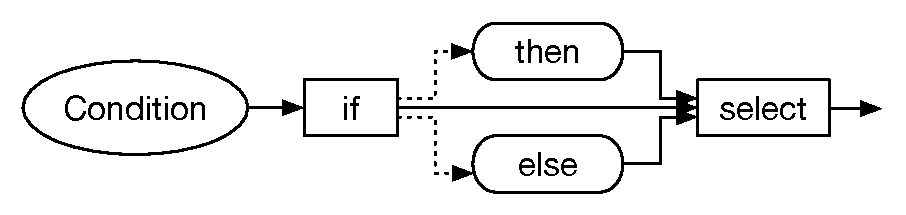
\includegraphics[width=\linewidth]{../Figures/if-in-operators}
    \caption{If represented in operators}
    \label{fig:if-in-operators}
\end{figure}

\subsection{Splitting branches}

\subsubsection{In code}

\begin{figure}
\begin{minted}{Haskell}
original :: Bool -> a
original cond =
    if cond
        then f
        else g

decomposed :: forall a b c => Bool -> a
decomposed cond =
    if cond
        then fAfter . first fetch . fBefore
        else gAfter . first fetch . gBefore
  where
    fBefore :: (FetchData, b)
    fBefore = -- omitted

    fAfter :: (FetchResult, b)
    fAfter = -- omitted

    gBefore :: (FetchData, c)
    gBefore = -- omitted

    gAfter :: (FetchResult, c)
    gAfter = -- omitted

splitIf :: forall a b c => Bool -> a
splitIf cond =
    ((if cond
        then fAfter . second fromLeft
        else gAfter . second fromRight)
        :: (FetchResult, Either b c) -> a)
    . (first fetch
      :: (FetchData, Either b c) -> (FetchResult, Either b c))
    ((if cond
        then second Left . fBefore
        else second Right . gBefore)
        :: (FetchData, Either b c))
  where
    fromLeft :: forall a b => Either a b -> a
    fromLeft = -- omitted

    fromRight :: forall a b => Either a b -> b
    fromRight = -- omitted
\end{minted}
\caption{Exemplary if rewrite in Haskell}
\label{fig:if-rewrite-in-code}
\end{figure}

We can apply a very similar method of decomposition as we did with smap.
To keep the transformation simple we assume both branches to have an equal number of fetches such that always two fetches, one from each branch, can be merged together.
If we merge one fetch from each branch we know that no matter the condition, exactly one of them is going to have input present.
Hence if we select whichever input is present and feed it to our single merged fetch it is guaranteed to have input no matter the condition.
Afterwards we will ensure the output from \fetch{} is fed back into the continuation of the branch the input came from.

In Figure~\ref{fig:if-rewrite-in-code} we can see an exemplary version of this rewrite in Haskell, again this is provided as a visual aid and an indicator for correctness as a result of the types lining up.
Again the idea is to decompose the original function into a part before and after the \fetch{}, as well as the \fetch{} itself.
Other data flowing between the before and after functions is packaged into a tuple with \texttt{FetchData} and \texttt{FetchResult} and the fetch is only applied to the data it concerns.

Intermediary we unify this free flowing data into an \texttt{Either} structure which is a sum data type, capable of holding one of of two arbitrary pieces of data since the free data flowing between \texttt{fBefore} $\rightarrow$ \texttt{fAfter} and \texttt{gBefore} $\rightarrow$ \texttt{gAfter} does not have to have the same type.

We later unpack this \texttt{Either} structure again, in a very non-typesafe way using \texttt{fromLeft} and \texttt{fromRight}.
However we can guarantee that this does not lead to errors because the condition is the same for both \texttt{if} expressions and \fetch{} only modifies the first part of the tuple, becuase of \texttt{first}.

\subsubsection{As dataflow graph}

As an exemplary graph in Figure~\ref{fig:if-trans-before} we see two branches, each with a fetch somewhere in them.
We cannot be sure which fetch gets executed when this code is run, however we know for certain that exactly one of them gets executed.
Therefore we insert a \texttt{select} operator into the graph which returns whichever input data was present and fetch that, see the red path in Figure~\ref{fig:if-trans-before} and \ref{fig:if-trans-merged}.
After that we wire the result into all places of the rest of \textbf{both} branches wherever one of the fetches was used.
We insert context arcs from the \texttt{if} operator to those places to make sure they run only if the respective branch was selected.
Any other data flow between the sections before and after the \texttt{fetch} are left unchanged, see the blue arrows in Figure~\ref{fig:if-trans-before} and \ref{fig:if-trans-merged}.

\begin{figure}
    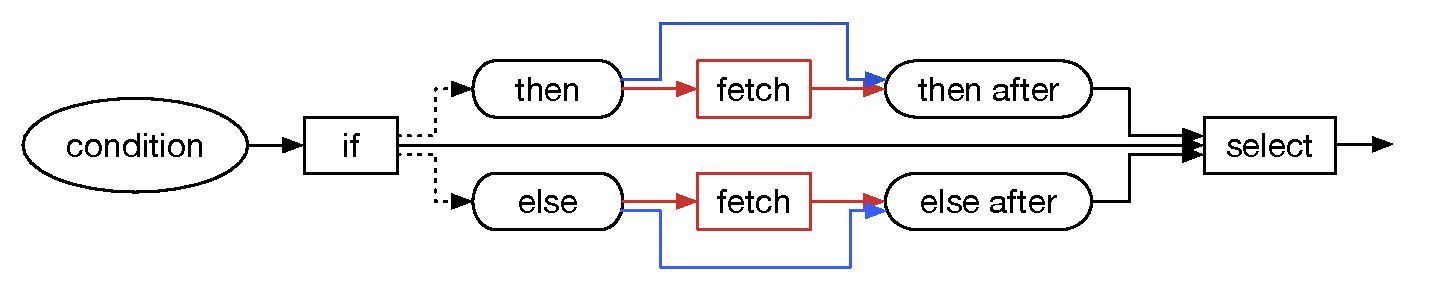
\includegraphics[width=\linewidth]{../Figures/if-trans-before}
    \caption{If transformation source graph}
    \label{fig:if-trans-before}
\end{figure}

\begin{figure}
    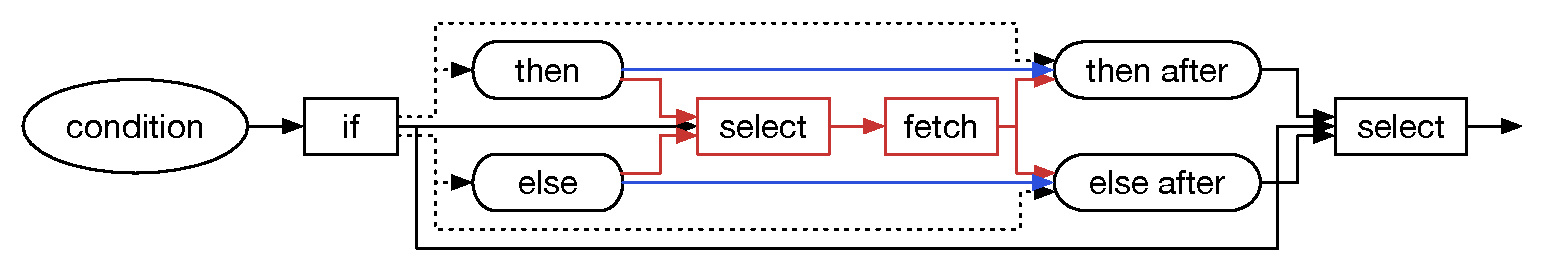
\includegraphics[width=\linewidth]{../Figures/if-trans-merged}
    \caption{If transformation after transformation}
    \label{fig:if-trans-merged}
\end{figure}

\subsection{Fetch imbalance}

We previously assumed that both branches held an equal number of fetches and that these could be paired up neatly in twos.
However in real programs this may not be the case at all, see Figure \ref{fig:if-insert-empty-parallel-before}.
There is a simple solution to this problem.
We solve the imbalance of fetches by inserting empty (NoOp) fetches at the front of the branch with fewer fetches, see Figure~\ref{fig:if-insert-empty-parallel-after}.

\begin{figure}
    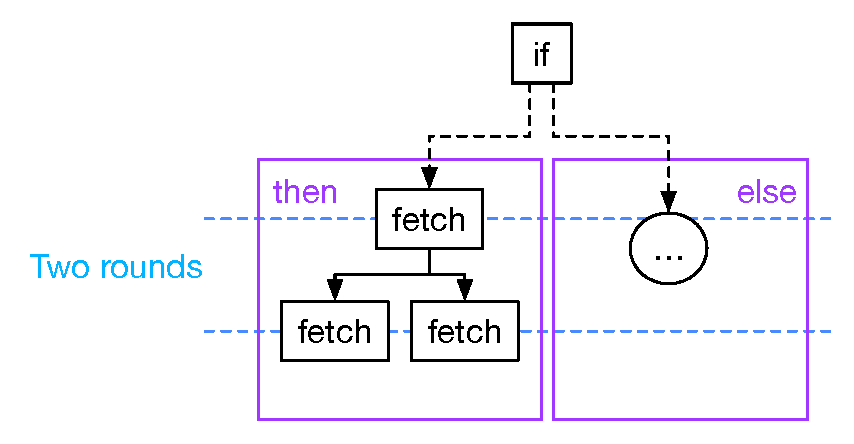
\includegraphics[width=\linewidth]{../Figures/if-insert-empty-parallel-before}
    \caption{Graph of a graph with imbalanced fetches in conditional}
    \label{fig:if-insert-empty-parallel-before}
\end{figure}

Originally I would create the empty fetches by collecting an graph of fetches and data dependencies between them on each branch.
From this I obtained a topologically sorted list of fetches.
After that I would calculate the difference in length between both lists to obtain a number of necessary empty fetches.
Then I would generate a sequence of request-fetch pairs as long as the calculated difference.
These would then be connected in sequence.
The first one would receive input from the last fetch of the shorter of the two previously calculated sequences of preexisting fetches.
An example of this can be seen in Figure~\ref{fig:if-insert-empty-parallel-after}.

Since these are NoOp they ignore their inputs, we use the inputs only to create data dependencies.
If the shorter sequence of preexisting fetches was empty a new operator \texttt{const-null} would be created and inserted.
This operator would not get input at all, except for a context arc from the \texttt{if} and emit a data packet containing \texttt{null} used to activating the first created fetch.
The second request-fetch pair would receive as input the result from the first fetch and the third one the result from the second and so on.
The final result was discarded.

\begin{figure}
    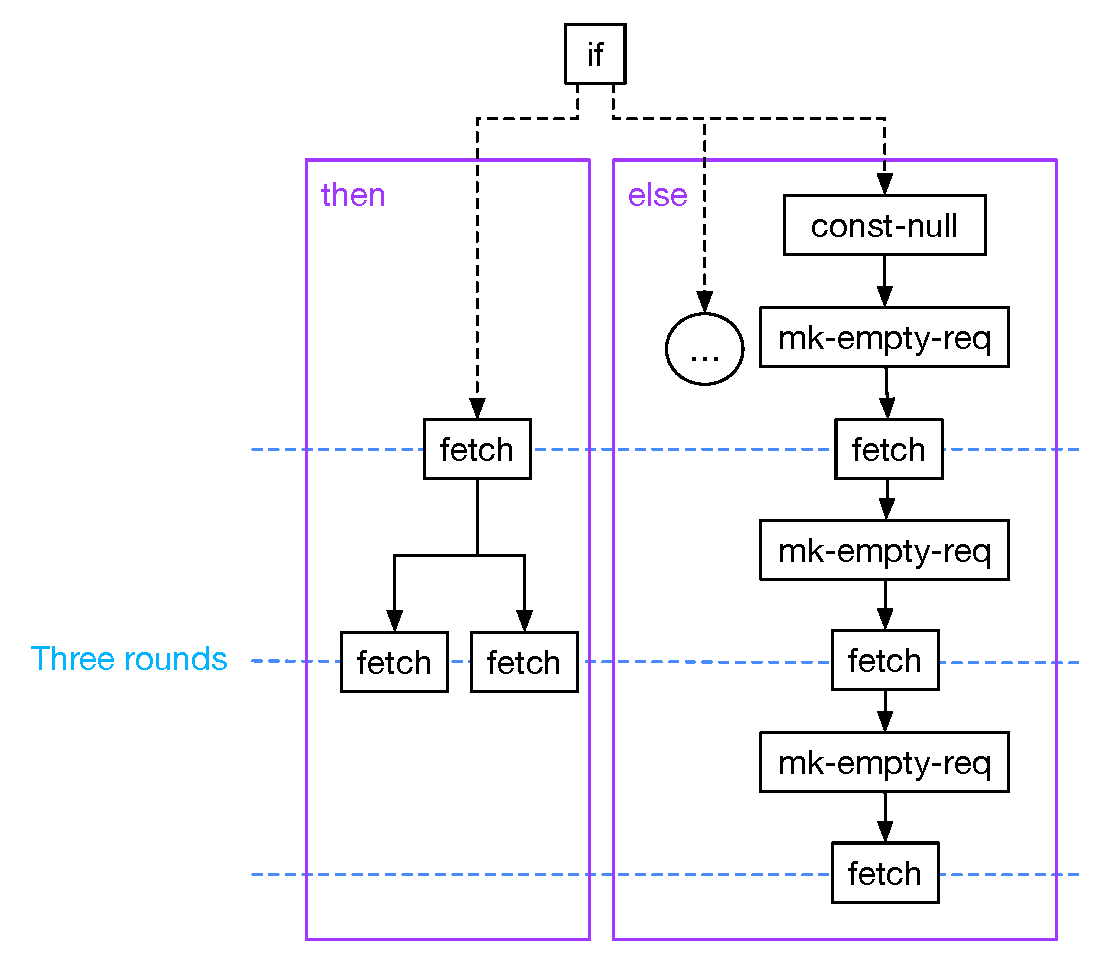
\includegraphics[width=\linewidth]{../Figures/if-insert-empty-parallel-after-insert}
    \caption{Insertion of empty requests and fetches}
    \label{fig:if-insert-empty-parallel-after}
\end{figure}

There is a significant problem with this approach, which is, and I only realised this late, that this created sequence is fully dependent.
Meaning each fetch depends on \textbf{all} of its predecessor fetches.
We have created a branch which contains a sequence of fully dependent fetches.
However there is no reason why the other, longer branch should be fully dependent also.
The result is that, once we merge both branches around the fetches the resulting combined fetches inherit both data dependencies.
Since you cannot depend on more than literally all predecessors the resulting merge inherits its dependence from the fully dependent second branch.
In the the second branch each fetch was dependent on all previous fetches in the branch, and from this follows that it will have to be in a separate fetch round to all its predecessors.
And since this is true for all fetches in the branch each of those will be in a separate round.
They can still be batched with other, parallel parts of the program, however we have lost the opportunity for some batching here, because we have forced sequentiality, even if it may not have existed originally.


There is a very simple solution to this problem, which, coincidentally, also simplified the implementation of the algorithm as a whole.
Now I only generate a single operator called \texttt{mk-empty-req} which creates one empty request, with no dependency other than the \texttt{if} operator.
Note that the \texttt{mk-empty-req} implementation changed as well to combine the functionality of \texttt{const-null} and the old \texttt{mk-empty-req}.
This empty request is the only argument to each of the NoOp fetches I create.
Therefore we only create one request, which reduces the number of operators, and the fetches depend only on the \texttt{mk-empty-req} and the \texttt{if} operator, not on one another.
Therefore they could in theory all be batched.
If we now merge the branches our empty requests will create no new dependencies, since they have the least dependency possible in the branch.

\begin{figure}
    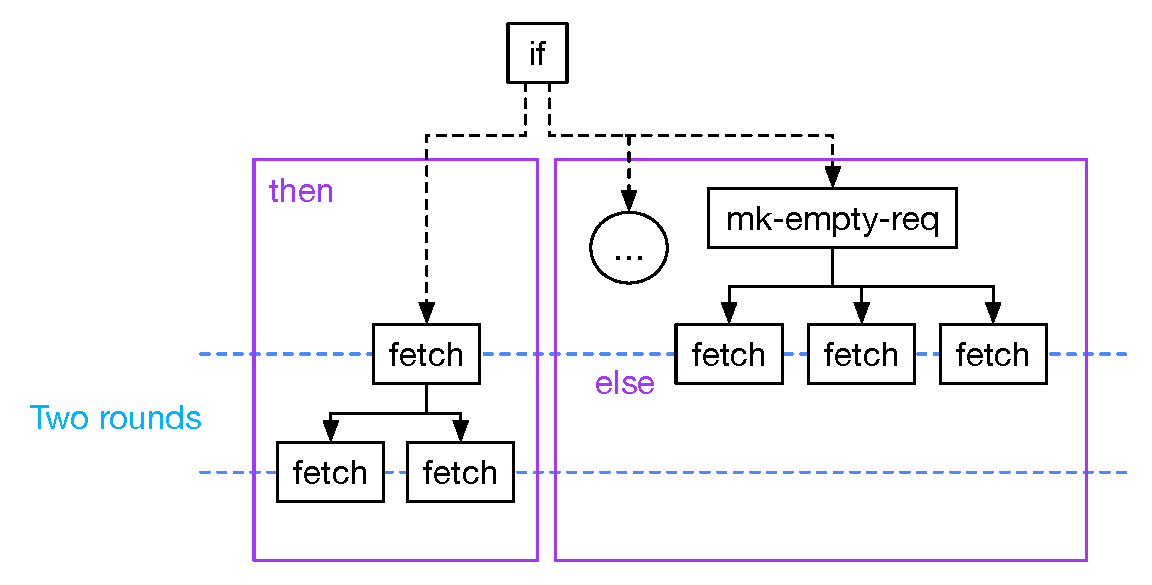
\includegraphics[width=\linewidth]{../Figures/if-insert-empty-better-after-insert}
    \caption{Better approach to empty requests and fetches}
    \label{if-insert-empty-better-after-insert}
\end{figure}

Now we can apply the merge transformation as described before.
